\documentclass[11pt]{article}
\usepackage[utf8]{inputenc}
\usepackage[spanish]{babel}
\usepackage[margin=2.5cm]{geometry}
\usepackage{graphicx}
\usepackage{listings}
\usepackage{xcolor}
\usepackage{hyperref}
\usepackage{amsmath}
\usepackage{float}

\definecolor{codebg}{RGB}{245,245,245}
\lstset{
  backgroundcolor=\color{codebg},
  basicstyle=\ttfamily\small,
  breaklines=true,
  frame=single,
  language=C++,
  columns=fullflexible,
  showstringspaces=false
}

\title{Avance Proyecto Final \\ \large Sistema de Animación de Océano}
\author{
  Princce Yorwin Mariños Hilario \\
  Gleddynuri Marbel Picha Chañi \\
  Wilson Ramos Pacco \\
  Postigo Cabana Juan Carlos
}
\date{Arequipa --- Perú \\ 2026}

\begin{document}

\begin{titlepage}
\centering
\vspace*{1cm}
{\large\bfseries UNIVERSIDAD NACIONAL DE SAN AGUSTÍN DE AREQUIPA}\\[0.3cm]
{\bfseries Facultad de Ingeniería de Producción y Servicios}\\
{\bfseries Escuela Profesional de Ciencia de la Computación}\\[2cm]

\vspace{1cm}
{\Huge\bfseries Avance Proyecto Final}\\[1cm]

\vspace{2cm}
\begin{flushleft}
\textbf{Docente:} Percy Maldonado Quispe \\[0.5cm]
\textbf{Alumnos:} \\
Princce Yorwin Mariños Hilario \\
Gleddynuri Marbel Picha Chañi \\
Wilson Ramos Pacco \\
Postigo Cabana Juan Carlos
\end{flushleft}

\vfill
\centering
Curso: Computación Gráfica \\
Arequipa --- Perú \\
2026
\end{titlepage}

\tableofcontents
\newpage

\section{Introducción y alcance de esta entrega}

Este documento presenta el avance correspondiente a la \textbf{Fase 1} del proyecto
\emph{Sistema de Animación de Océano}: generación de la malla base y animación de
oleaje mediante superposición de ondas sinusoidales (modelo de Gerstner/suma de senos).
Quedan fuera del alcance de esta entrega, y se abordarán en fases posteriores, el
cálculo de normales para iluminación, el mapeo de texturas y el control interactivo
de cámara.

\section{Organización y configuración del entorno}

Para mantener el proyecto escalable, el código se organiza en una estructura de
directorios separando fuentes, cabeceras y recursos:

\begin{lstlisting}[language=bash]
VisualizacionOcean/
|
+-- src/
|   +-- main.cpp
|   +-- Ocean.cpp
|   +-- Wave.cpp
|
+-- include/
|   +-- Ocean.h
|   +-- Wave.h
|   +-- WPoint.h
|
+-- assets/
|   +-- textures/
|       +-- ocean.tga
|
+-- data/
    +-- spectrum.txt
\end{lstlisting}

Se inicializó el control de versiones con Git y se configuró un \texttt{.gitignore}
para excluir binarios y artefactos de compilación.

\section{Arquitectura del sistema}

El sistema se organiza en tres clases con responsabilidades separadas:

\subsection{WPoint --- el vértice}

Unidad básica de la malla. Almacena posición, normal (reservada para la fase de
iluminación) y coordenadas UV (reservadas para la fase de texturizado).

\begin{lstlisting}
struct WPoint {
    float x, y, z;       // Posicion en el espacio
    float nx, ny, nz;     // Vector normal
    float s, t;           // Coordenadas de textura UV
};
\end{lstlisting}

\subsection{Wave --- la ola}

Encapsula los parámetros físicos de una ola individual: amplitud, frecuencia,
dirección y fase. Provee el cálculo del número de onda $k$, necesario para la
fórmula de desplazamiento:

\[
k = \frac{4\pi^2 f^2}{g}, \qquad g = 9.81 \; \text{m/s}^2
\]

\begin{lstlisting}
class Wave {
    float amplitude, frequency, direction, phase;
public:
    Wave(float amp, float freq, float dir, float ph);
    float getWaveNumber() const; // Calcula k
};
\end{lstlisting}

\subsection{Ocean --- el controlador}

Administra la malla 2D de vértices, la lista de olas cargadas desde
\texttt{data/spectrum.txt} y las operaciones de ciclo de vida (actualización,
cálculo de normales y dibujo).

\begin{lstlisting}
class Ocean {
private:
    std::vector<std::vector<WPoint>> mesh;
    std::vector<Wave> waves;
public:
    void initMesh();
    bool loadWaves(const std::string& filename);
    void update(float time);
    void draw();
};
\end{lstlisting}

\section{Generación de la malla base}

Se implementó la lógica para construir la base del océano sobre el plano $XZ$.
La cuadrícula se centra dinámicamente respecto al origen para quedar bien
posicionada frente a la cámara; todos los vértices inician con altura $y=0$ y
normal apuntando hacia arriba, listos para ser deformados en la etapa de
animación.

\begin{lstlisting}
void Ocean::initMesh() {
    mesh.resize(rows, std::vector<WPoint>(cols));

    float startX = -((cols - 1) * spacing) / 2.0f;
    float startZ = -((rows - 1) * spacing) / 2.0f;

    for (int i = 0; i < rows; ++i) {
        for (int j = 0; j < cols; ++j) {
            mesh[i][j].x = startX + j * spacing;
            mesh[i][j].y = 0.0f;
            mesh[i][j].z = startZ + i * spacing;
            mesh[i][j].s = (float)j / (cols - 1);
            mesh[i][j].t = (float)i / (rows - 1);
        }
    }
}
\end{lstlisting}

\section{Renderizado en modo alambre}

Para validar visualmente que la topología de la superficie es correcta antes de
introducir desplazamiento vertical, iluminación o texturas, se renderiza la malla
en modo alambre (\texttt{GL\_LINE}) usando GLUT.

\begin{lstlisting}
void Ocean::draw() {
    glPolygonMode(GL_FRONT_AND_BACK, GL_LINE);

    glBegin(GL_TRIANGLES);
    for (int i = 0; i < rows - 1; ++i) {
        for (int j = 0; j < cols - 1; ++j) {
            glVertex3f(mesh[i][j].x,     mesh[i][j].y,     mesh[i][j].z);
            glVertex3f(mesh[i+1][j].x,   mesh[i+1][j].y,   mesh[i+1][j].z);
            glVertex3f(mesh[i][j+1].x,   mesh[i][j+1].y,   mesh[i][j+1].z);

            glVertex3f(mesh[i][j+1].x,   mesh[i][j+1].y,   mesh[i][j+1].z);
            glVertex3f(mesh[i+1][j].x,   mesh[i+1][j].y,   mesh[i+1][j].z);
            glVertex3f(mesh[i+1][j+1].x, mesh[i+1][j+1].y, mesh[i+1][j+1].z);
        }
    }
    glEnd();

    glPolygonMode(GL_FRONT_AND_BACK, GL_FILL);
}
\end{lstlisting}

 \begin{figure}[H]
 \centering
 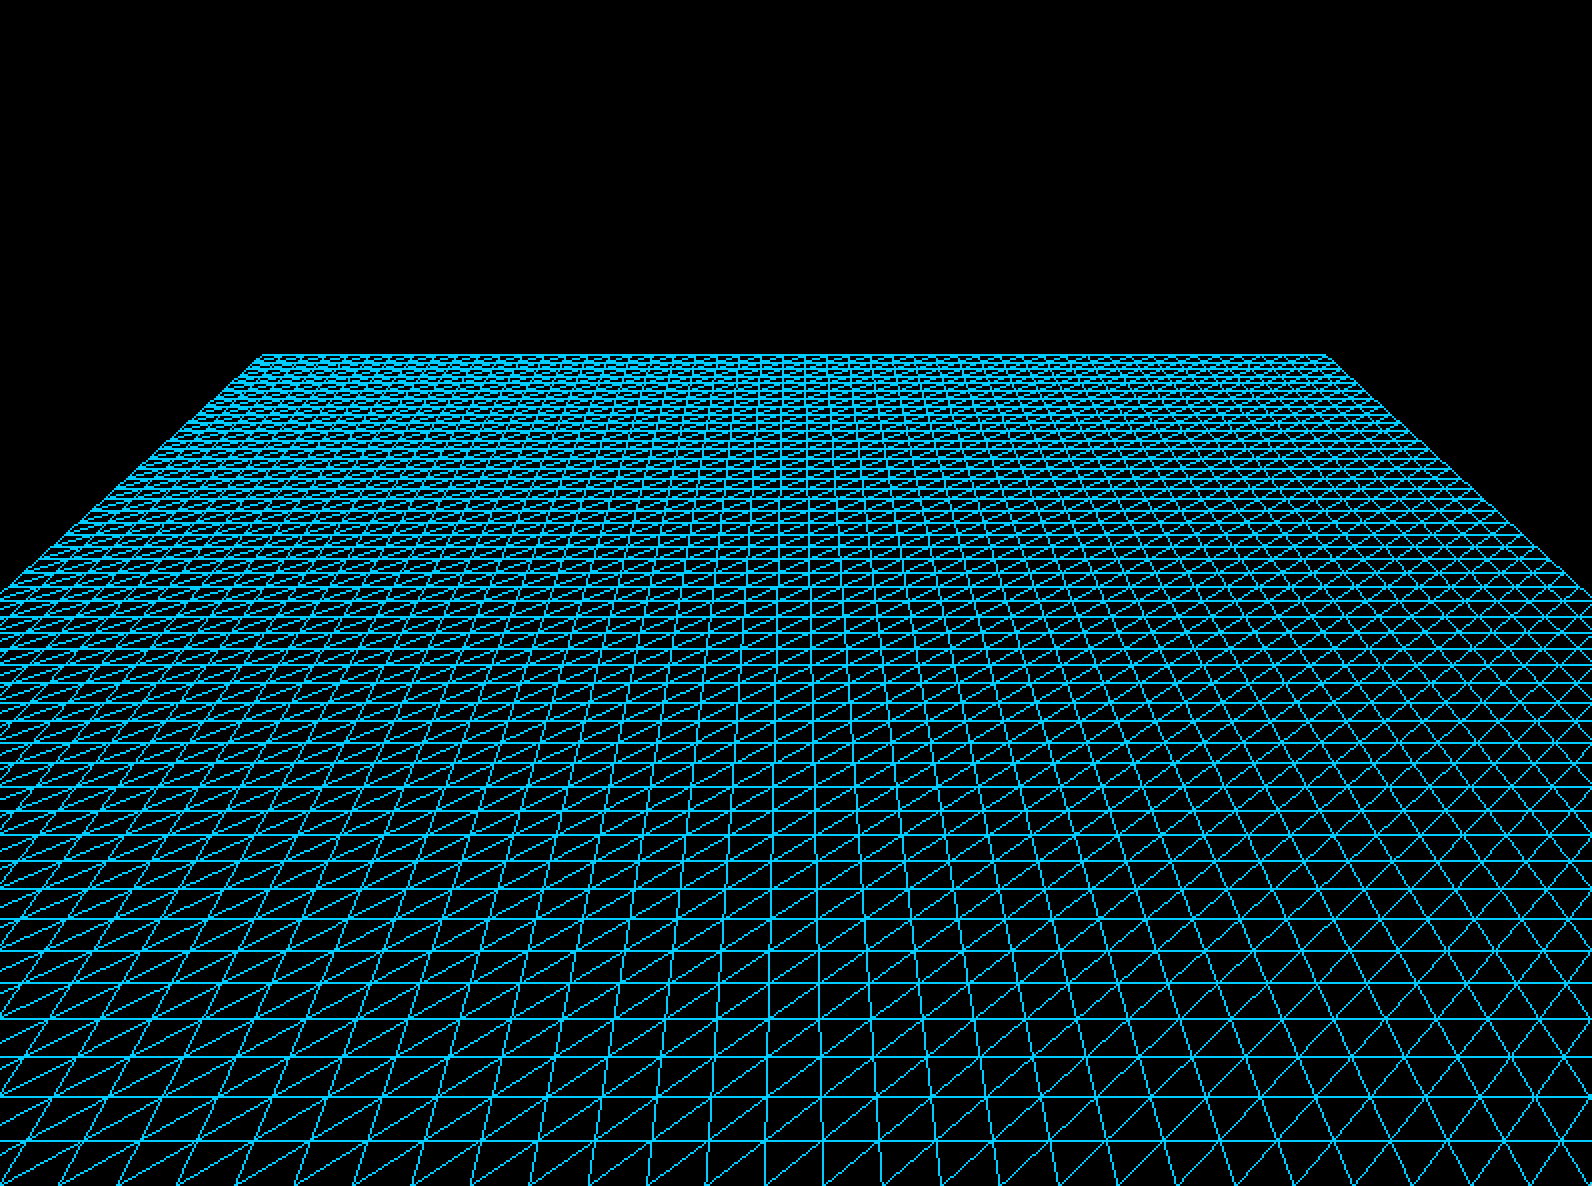
\includegraphics[width=0.8\textwidth]{figuras/malla_plana_alambre.png}
 \caption{Malla base plana renderizada en modo alambre, estado real del código en este avance.}
 \end{figure}

\section{Estado pendiente de esta fase}

Al cierre de esta entrega, las siguientes piezas están declaradas en la interfaz
pero aún no implementadas (retornan valores por defecto o cuerpos vacíos):

\begin{itemize}
  \item \texttt{Ocean::loadWaves()}: falta parsear \texttt{data/spectrum.txt} y
        construir el vector de objetos \texttt{Wave}.
  \item \texttt{Ocean::update(float time)}: falta aplicar la suma de senos de
        todas las olas cargadas sobre la coordenada $y$ de cada vértice.
  \item \texttt{main.cpp}: falta un \texttt{glutIdleFunc} o
        \texttt{glutTimerFunc} que avance el tiempo de simulación y solicite
        redibujado; actualmente el océano no se anima.
  \item \texttt{Ocean::loadTexture()} y \texttt{Ocean::computeNormals()}:
        reservados para las fases de iluminación y texturizado, fuera del
        alcance de este avance.
\end{itemize}

Estas piezas conforman el trabajo pendiente para cerrar formalmente la Fase 1.

\section{Conclusiones parciales}

Se cuenta con una arquitectura orientada a objetos clara y con la generación de
la malla base validada visualmente en modo alambre. El siguiente paso inmediato
es implementar la carga del espectro de olas y la función de actualización
temporal para lograr la primera animación visible del oleaje, antes de avanzar
a iluminación y texturizado en fases posteriores.

\end{document}
